\documentclass[tikz,border=10pt]{standalone}
% Shared preamble for the CenterTask panel files (panel_a/b/c.tex).
% Edit colours and node styles here, once.
\usepackage{amsmath}
\usetikzlibrary{arrows.meta,positioning,calc}

% category colours as in ColorCategoryMap.m: 1=Short/Orange, 2=Mid/Green, 3=Long/Blue
\definecolor{catShort}{RGB}{243,178,132}
\definecolor{catMid}{RGB}{158,209,172}
\definecolor{catLong}{RGB}{157,188,234}

\tikzset{ctpanel/.style={
  font=\sffamily,
  band/.style={rounded corners=6pt, fill=black!7, draw=none, inner sep=8pt, minimum height=1.15cm},
  unit/.style={circle, fill=catMid!60, draw=none, minimum size=0.95cm, inner sep=0pt},
  flow/.style={-{Latex[length=2.2mm]}, line width=0.8pt},
  rowlab/.style={anchor=east, font=\sffamily\large},
  now/.style={fill=catShort!55, rounded corners=3pt, inner sep=3pt},
  stage/.style={rounded corners=6pt, fill=black!8, draw=none, inner sep=8pt, minimum height=1.2cm, align=center},
  target/.style={circle, minimum size=0.9cm, inner sep=0pt, draw=none, font=\sffamily\scriptsize, text=black!75},
  axis/.style={line width=0.6pt},
}}

\usetikzlibrary{shapes.misc}

% ---------------------------------------------------------------------
%  On-screen trial sequence (CenterOutTask.m), 3-category framing.
%  Epoch order follows TaskEpoch.m's execution-order comment:
%    ENTER_CENTER -> HOLD -> BAR -> CUE -> DECISION_TIME -> MOVEMENT ->
%    TARGET_HOLD -> REWARD/SUCCESS_FB (or ERROR_FB) -> ITI
%  Default durations (s) from ConfigOrgParams.m: hold ~1.0-1.5 (holdTimeBase
%  + holdTimeDelta), bar 1.0 (barDuration), cue 0.5 (cueDuration), decision
%  <=2 (maxDecisionTime), execution <=2.5 (maxExecutionTime), target hold
%  0.05 (minTarHoldTime), feedback 0.2 (tarHoldFeed/tarErrorFeed), ITI
%  2.0+-0.5 (ITI/ITIDelta). STIM_DELAY/CUE_DELAY omitted: both default to 0
%  and are not entered on a standard trial (see TaskEpoch.m).
% ---------------------------------------------------------------------

\begin{document}
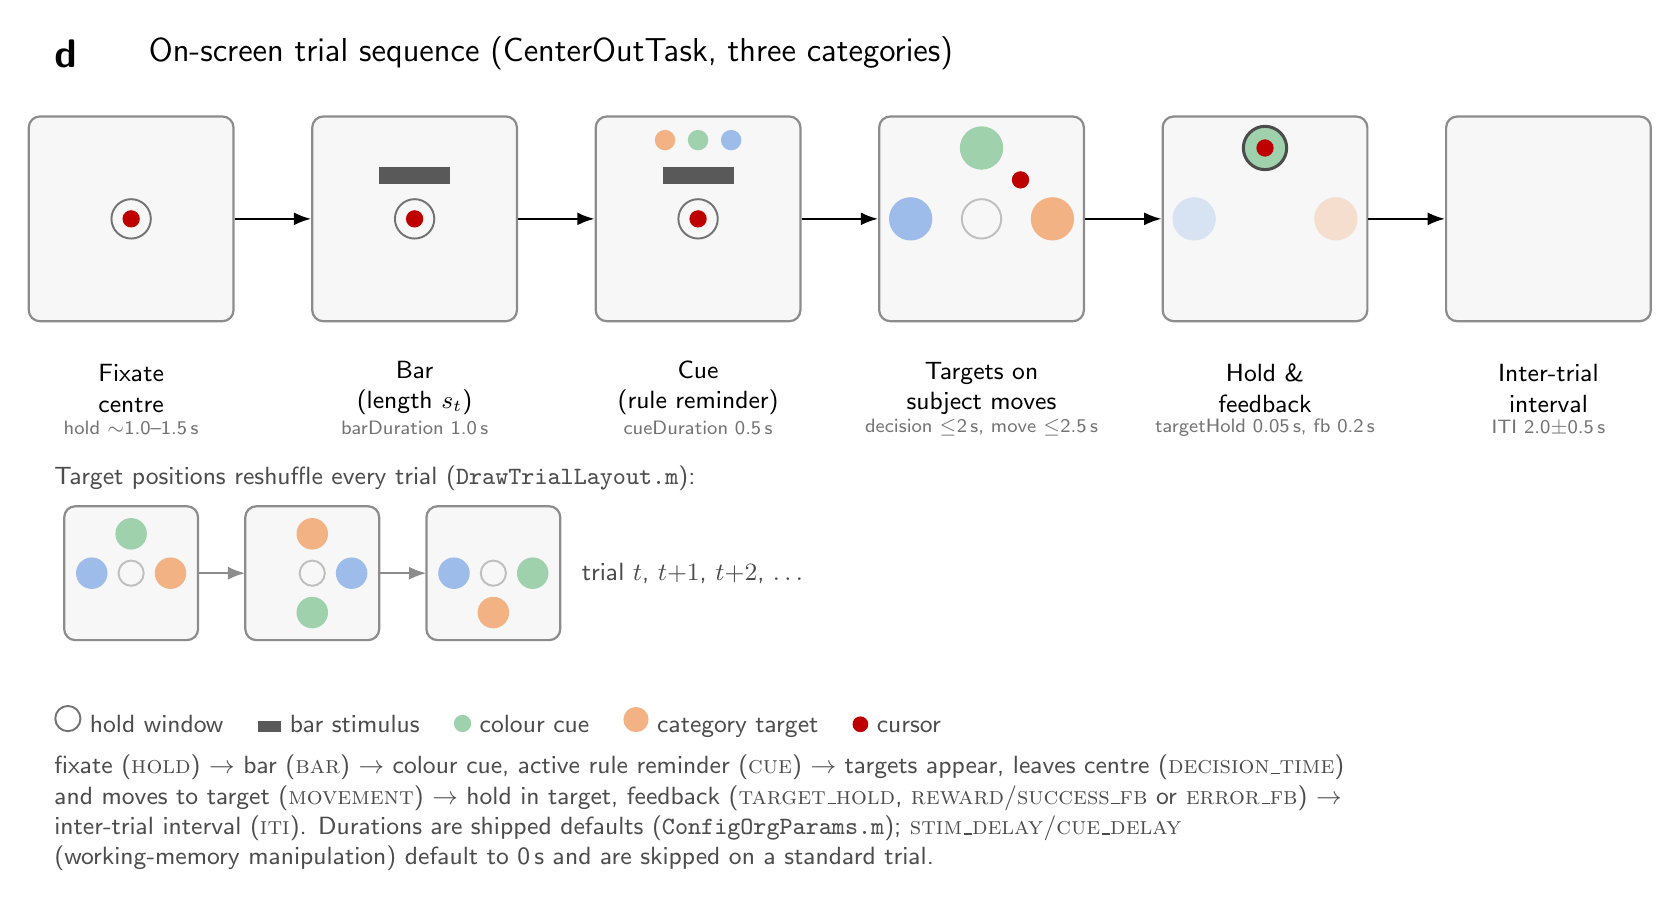
\begin{tikzpicture}[
  font=\sffamily,
  screen/.style={rounded corners=4pt, draw=black!45, line width=0.8pt, fill=black!3,
                 minimum width=2.6cm, minimum height=2.6cm},
  capt/.style={font=\sffamily\small, align=center},
  timelab/.style={font=\sffamily\scriptsize, text=black!55},
  arrowlab/.style={-{Latex[length=1.8mm]}, line width=0.7pt, black!55},
  cursor/.style={circle, fill=red!75!black, draw=none, minimum size=2.2mm, inner sep=0pt},
  flow/.style={-{Latex[length=2.2mm]}, line width=0.8pt},
  hold/.style={circle, draw=black!55, line width=0.7pt, fill=none},
  cuecirc/.style={circle, minimum size=2.6mm, inner sep=0pt},
  targ/.style={circle, minimum size=5.5mm, inner sep=0pt, draw=none},
]

% common geometry inside each 2.6x2.6cm screen (local coords, centre = 0,0)
\def\holdR{2.5mm}
\def\barW{9mm}
\def\barH{2.2mm}
\def\tgtR{9mm}     % distance from centre to each cardinal target

% ===================================================================
% Panel label + title
% ===================================================================
\node[font=\sffamily\bfseries\Large, anchor=west] at (-1.1,2.1) {d};
\node[font=\sffamily\large, anchor=west] at (0.1,2.1) {On-screen trial sequence (CenterOutTask, three categories)};

% ===================================================================
% helper: draw one screen frame at (x,y) with given contents
% ===================================================================

% ---------- 1. ENTER_CENTER / HOLD ----------
\begin{scope}[xshift=0cm]
  \node[screen] (S1) at (0,0) {};
  \draw[hold] (S1) circle (\holdR);
  \node[cursor] at (S1) {};
  \node[capt] at (0,-2.15) {Fixate \\ centre};
  \node[timelab] at (0,-2.65) {hold $\sim$1.0--1.5\,s};
\end{scope}

% ---------- 2. BAR ----------
\begin{scope}[xshift=3.6cm]
  \node[screen] (S2) at (0,0) {};
  \draw[hold] (S2) circle (\holdR);
  \node[cursor] at (S2) {};
  \fill[black!65] ($(S2)+(0,0.55)$) ++(-\barW/2,-\barH/2) rectangle ++(\barW,\barH);
  \node[capt] at (0,-2.15) {Bar \\ (length $s_t$)};
  \node[timelab] at (0,-2.65) {barDuration 1.0\,s};
\end{scope}

% ---------- 3. CUE ----------
\begin{scope}[xshift=7.2cm]
  \node[screen] (S3) at (0,0) {};
  \draw[hold] (S3) circle (\holdR);
  \node[cursor] at (S3) {};
  \fill[black!65] ($(S3)+(0,0.55)$) ++(-\barW/2,-\barH/2) rectangle ++(\barW,\barH);
  \node[cuecirc, fill=catShort] at ($(S3)+(-0.42,1.0)$) {};
  \node[cuecirc, fill=catMid]   at ($(S3)+(0,1.0)$) {};
  \node[cuecirc, fill=catLong]  at ($(S3)+(0.42,1.0)$) {};
  \node[capt] at (0,-2.15) {Cue \\ (rule reminder)};
  \node[timelab] at (0,-2.65) {cueDuration 0.5\,s};
\end{scope}

% ---------- 4. DECISION_TIME / MOVEMENT (targets placed, subject moves out) ----------
\begin{scope}[xshift=10.8cm]
  \node[screen] (S4) at (0,0) {};
  \draw[hold, black!25] (S4) circle (\holdR);
  \node[targ, fill=catMid]   at ($(S4)+(0,\tgtR)$)   {};
  \node[targ, fill=catShort] at ($(S4)+(\tgtR,0)$)   {};
  \node[targ, fill=catLong]  at ($(S4)+(-\tgtR,0)$)  {};
  \node[cursor] at ($(S4)+(0.55*\tgtR,0.55*\tgtR)$) {};
  \node[capt] at (0,-2.15) {Targets on \\ subject moves};
  \node[timelab] at (0,-2.65) {decision $\le$2\,s, move $\le$2.5\,s};
\end{scope}

% ---------- 5. TARGET_HOLD / feedback ----------
\begin{scope}[xshift=14.4cm]
  \node[screen] (S5) at (0,0) {};
  \node[targ, fill=catMid, draw=black!70, line width=1.1pt]   at ($(S5)+(0,\tgtR)$)   {};
  \node[targ, fill=catShort, opacity=0.35] at ($(S5)+(\tgtR,0)$)   {};
  \node[targ, fill=catLong, opacity=0.35]  at ($(S5)+(-\tgtR,0)$)  {};
  \node[cursor] at ($(S5)+(0,\tgtR)$) {};
  \node[capt] at (0,-2.15) {Hold \& \\ feedback};
  \node[timelab] at (0,-2.65) {targetHold 0.05\,s, fb 0.2\,s};
\end{scope}

% ---------- 6. ITI ----------
\begin{scope}[xshift=18.0cm]
  \node[screen] (S6) at (0,0) {};
  \node[capt] at (0,-2.15) {Inter-trial \\ interval};
  \node[timelab] at (0,-2.65) {ITI 2.0$\pm$0.5\,s};
\end{scope}

% ===================================================================
% flow arrows between screens
% ===================================================================
\foreach \a/\b in {S1/S2, S2/S3, S3/S4, S4/S5, S5/S6}{
  \draw[flow] (\a.east) -- (\b.west);
}

% ===================================================================
% inset: target-position reshuffling across trials (DrawTrialLayout.m
% shuffles which cardinal direction/colour each category lands on every
% trial, so the same stimulus is not solved by spatial memory)
% ===================================================================
\node[font=\sffamily\small, anchor=west, text=black!70] at (-1.1,-3.3)
  {Target positions reshuffle every trial (\texttt{DrawTrialLayout.m}):};

\def\miniR{5.0mm}   % mini-screen target radius
\newcommand{\minilayout}[4]{%
  % #1 = centre coordinate, #2/#3/#4 = angle (deg) for Short/Mid/Long targets
  \node[screen, minimum width=1.7cm, minimum height=1.7cm] (M) at (#1) {};
  \draw[hold, black!25] (M) circle (1.6mm);
  \node[targ, minimum size=4mm, fill=catShort] at ($(M)+({#2}:\miniR)$) {};
  \node[targ, minimum size=4mm, fill=catMid]   at ($(M)+({#3}:\miniR)$) {};
  \node[targ, minimum size=4mm, fill=catLong]  at ($(M)+({#4}:\miniR)$) {};
}
\minilayout{0.0,-4.5}{0}{90}{180}
\minilayout{2.3,-4.5}{90}{270}{0}
\minilayout{4.6,-4.5}{270}{0}{180}
\node[font=\sffamily\small, anchor=west, text=black!70] at (5.6,-4.5)
  {trial $t$, $t{+}1$, $t{+}2$, $\ldots$};
\draw[flow, black!45] (0.85,-4.5) -- (1.45,-4.5);
\draw[flow, black!45] (3.15,-4.5) -- (3.75,-4.5);

% ===================================================================
% legend
% ===================================================================
\node[align=left, anchor=north west, font=\sffamily\small, text=black!70] at (-1.1,-6.05) {%
  \tikz{\draw[hold] (0,0) circle (1.6mm);} hold window \quad
  \tikz{\fill[black!65] (0,-0.7mm) rectangle (3mm,0.7mm);} bar stimulus \quad
  \tikz{\node[cuecirc, fill=catMid, minimum size=2.2mm] at (0,0) {};} colour cue \quad
  \tikz{\node[targ, fill=catShort, minimum size=3.2mm] at (0,0) {};} category target \quad
  \tikz{\node[cursor, minimum size=2mm] at (0,0) {};} cursor\\[4pt]
  fixate (\textsc{hold}) $\rightarrow$ bar (\textsc{bar}) $\rightarrow$ colour cue, active rule
  reminder (\textsc{cue}) $\rightarrow$ targets appear, leaves centre (\textsc{decision\_time})\\
  and moves to target (\textsc{movement}) $\rightarrow$ hold in target, feedback
  (\textsc{target\_hold}, \textsc{reward}/\textsc{success\_fb} or \textsc{error\_fb}) $\rightarrow$\\
  inter-trial interval (\textsc{iti}). Durations are shipped defaults (\texttt{ConfigOrgParams.m});
  \textsc{stim\_delay}/\textsc{cue\_delay}\\
  (working-memory manipulation) default to 0\,s and are skipped on a standard trial.
};

\end{tikzpicture}
\end{document}
